\documentclass{article}
\usepackage{amsmath, amssymb, amsthm, graphicx}
\usepackage[export]{adjustbox}

\title{Chapter 2 Section 2}
\author{Andrew Taylor}
\date{April 6 2022}
\newtheorem{theorem}{Theorem}
\newtheorem{problem}{Problem}
\newtheorem*{solution}{Solution}

\begin{document}
\maketitle

The letter L can be represented by the vectors $(0, 2)$ and $(1, 0)$. 

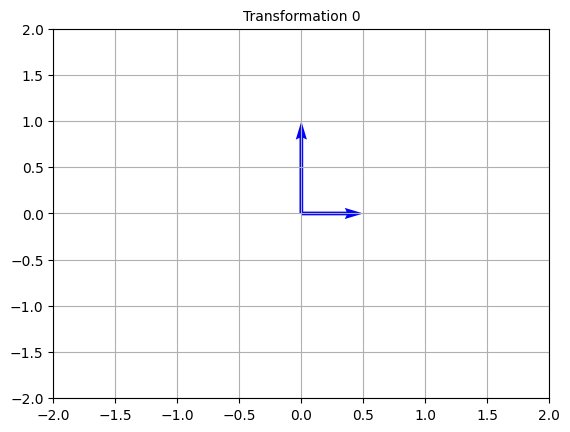
\includegraphics[width=5cm, height=5cm, center]{ch2sec2fig0} 

The following problems ask for a linear transformation of the letter L. In the following problems, give the matrix of the transformation and plot the result.

\begin{problem}
Scale L by a factor of $\displaystyle \frac{1}{2}$
\end{problem}

\begin{solution}
The matrix of the transformation is 

\begin{align*}
\begin{bmatrix}
0.5 & 0.0 \\ 
0.0 & 0.5
\end{bmatrix}
\end{align*}

After the scaling, the L looks like this

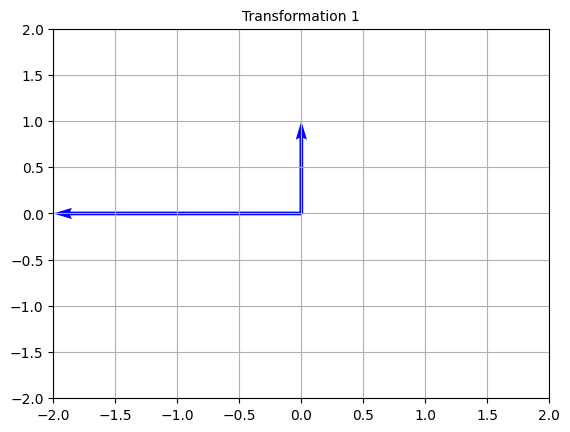
\includegraphics[width=5cm, height=5cm, center]{ch2sec2fig1} 

Note that in creating this shape, we scaled both vectors that make up the L.

\end{solution}

\end{document}